\documentclass[prb,preprint]{revtex4-1} 
\raggedbottom
\usepackage{amsmath}
\usepackage{amsfonts}
\usepackage{graphicx}

\begin{document}

\title{Studying The Nature of Radiation}

\author{Ryan S. Morshead}

\affiliation{Department of Physics, California State Polytechnic University}

\date{\today}

\begin{abstract}
Using a photomultiplier tube (PMT) and a multichannel analyzer (MCA) we analyzed the energy of gamma-rays produced in the radioactive isotopes $^{57}$Co, $^{137}$Cs, $^{22}$Na, and $^{60}$Co in addition to another unknown Isotope which we sought to identify. Following calibration procedures, the photopeak energies for these elements, reported in keV, were found to be 113$\pm9$, 659$\pm2$, 1275.1$\pm0.1$, 1169$\pm3$, and 829$\pm3$ respectively. Their corresponding accepted values, also reported in keV, are 122.1, 661.7, 1275.0, and 1173.2 with the exception of the unknown. A comparison of these values, again with the exception of the unknown, shows that all the measured values are in agreement with their accepted counterparts. More data on $^{137}$Cs showed that the full width at half maximum of its photopeak was 46$\pm6$ keV, that it had a Compton edge of 469$\pm3$ keV, and a secondary peak energy of 220$\pm8$ keV. The theoretical Compton edge value of 474.772$\pm0.001$ keV is shown to be in agreement with the measured value presented here. Identifying the source of the second peak energy involved calculating the angle of the incident gamma-rays which would produce that peak. This angle was calculated to be 122.97$\pm0.02$ degrees, confirming that this peak results from Compton backscattering. Additionally, the resolution of the photopeak on $^{137}$Cs was calculated to be 0.070$\pm0.002$ and the resolution of $^{60}$Co's photopeak was found to be 0.065$\pm0.001$. Finally, using the 8th edition of the table of isotopes which was last updated in 1999, to compare the known and measured photopeak energies, a single likely candidate was found to match the energy spectrum of the unidentified isotope. The known photopeak for $^{54}$Mn is 834.848 keV while the measured photopeak of unknown, listed above, was 829$\pm3$ keV. In comparing the two values we find that the photopeak energy for the identified element in the table of isotopes is in agreement with our own measured value for the unknown isotope.


\end{abstract}


\maketitle


\section{Introduction}
In 1895 Wilhelm Roentgen was working with a device which discharged x-rays at a target inside an evacuated glass tube. While working with this device he noticed that some platino-barium cyanide crystals, which he just happened to have close by, began to glow -- and that they stopped glowing when he switched the device off. Roentgen had accidentally discovered a new form of radiation. He had also accidentally discovered materials that could be used to produce a scintillator radiation detector.

Though scintillators are often used for the detection of ionizing radiation today, the first deep analysis of radioactive materials by Marie Curie in 1888 used a simple ionization chambers based upon a parallel-plate condenser in conjunction with an electrometer instead \cite{curie}. The creation of the photomultiplier tube in the 1940's and the discovery of scintillation in naphthalene led to new era in the development of scintillator detectors. This period began with Hoftadter's development of the thallium activated NaI. In a burst of exploration during the following years, the scintillation properties of most pure and activated alkali halide crystals were investigated \cite{R}. Unfortunately though, the detectors that Kallmann's work implied weren't possible until 1960 when silicon and germanium were available in sufficient sizes. Once they were implemented though they provided much high counting resolution. In the ensuing decades a steady progression of new scintillator material were discovered, including core-valence luminescence. 

The work done in this paper utilizes scintillators to examine the radioactivity of different materials with improved resolution as compared to what was allowed by the devices used in the late 18$^{th}$ century.

\newpage

\section{Experimental Design}

\subsection{Apparatus}
The arrangement required to observe and analyze gamma-ray photons, and thereby the radioactive materials which produce them, consists of a (PMT), NaI scintillation crystal, linear amplifier, oscilloscope and an (MCA). The system, shown in Fig. \ref{s}, operates the MCA as a pulse height analyzer. The photomultiplier tube converts photons into the form of an electric current and uses a light sensitive cathode, several electrodes, and an anode from which the final signal is drawn to do so. A photon which interacts with the cathode and releases an electron from the material will create a cascade of electrons which increase in number as they move from one electrode to the next. By the time the resulting cloud of electrons reaches the anode they number $\approx10^5$. Thus a measurable current pulse is created which is proportional to the original number of photons that hit the anode. Additionally, because the current originally results from a single photon the gain of the PMT can be said to be $\approx10^5$.

\begin{figure}[h!]
\centering
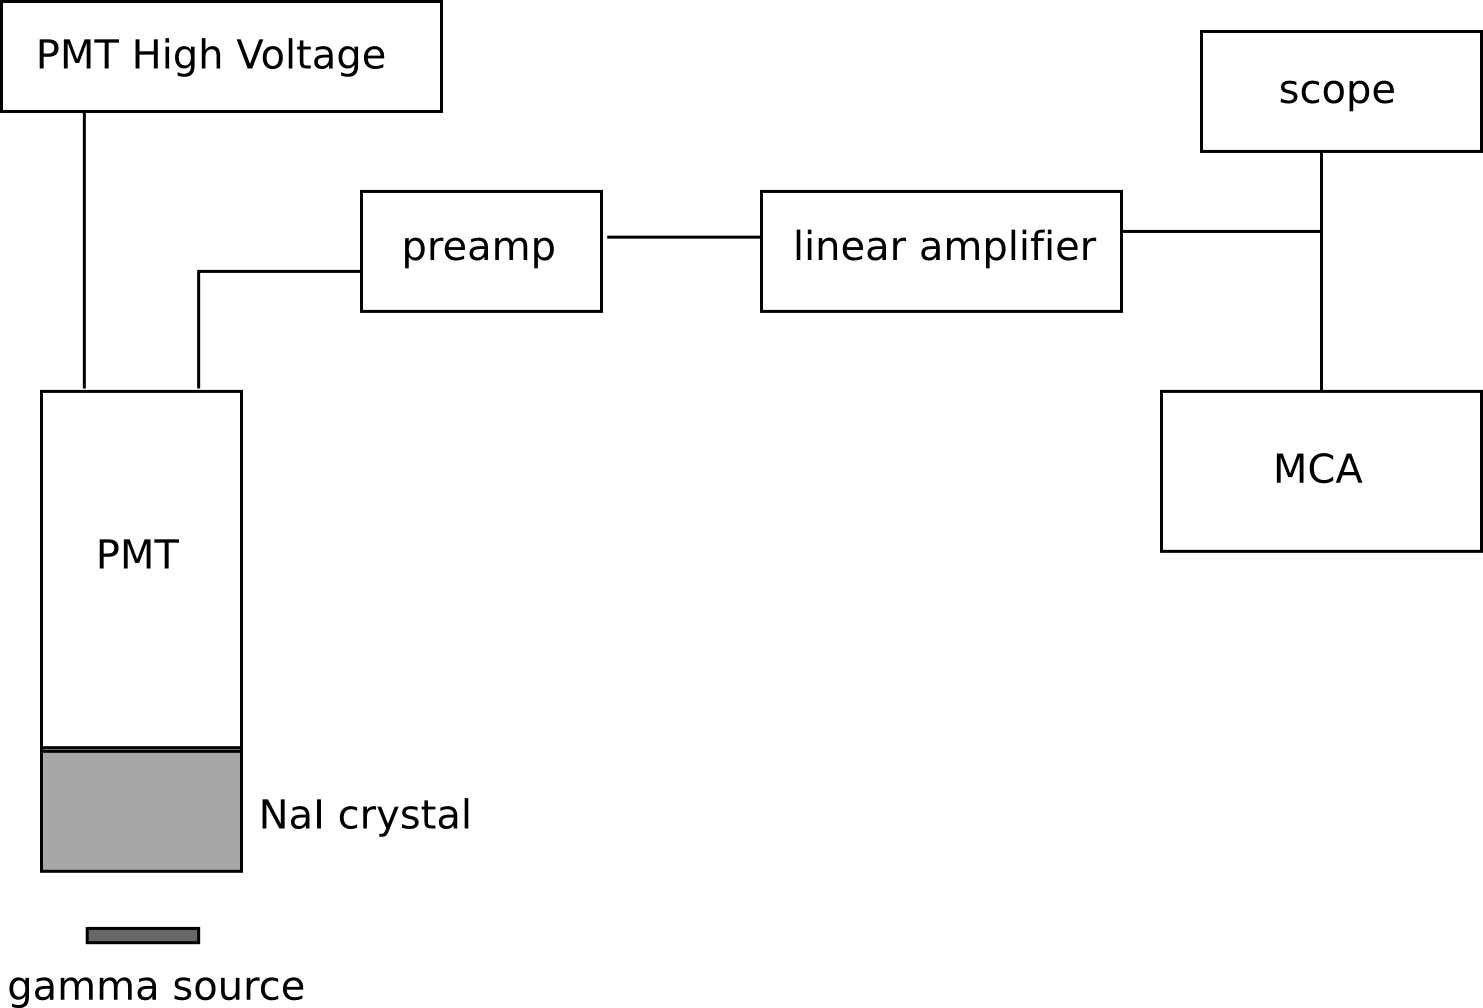
\includegraphics[width=.65\textwidth]{Scintillation.png}
\caption{Block diagram of the experimental system}
\label{s}
\end{figure}

\subsection{Measurement of $^{57}$Co, $^{137}$Cs, $^{2}$Na, $^{60}$Co and the Unknown Isotope}
We do not directly measure the gamma-rays generated by decays in the $^{57}$Co, $^{137}$Cs, $^{2}$Na, and $^{60}$Co samples as well as the unknown isotope. Instead we measure the scintillation produced when they interact with a scintillator crystal. Because of this we must account for artifacts which Compton scattering introduces to the voltage read-out from the PMT.

There are four possible interactions that a gamma-ray can have with an electron in the scintillator crystal. In the case of a photoelectric interaction, the energy of the electron, $E_{elec}$, equals the energy of the gamma-ray, $E_{\gamma}$. But that can only be said because the binding energy of the material is negligible. Additionally this kind of interaction will contribute to a peak in the energy spectrum called the photopeak.

Though Compton scattering produces electrons that have less energy than $E_\gamma$ in the case where a gamma-ray scatters of one or more electrons the total energy of the gamma-ray is maintained within the system. As a result this kind of interaction still adds to the photopeak. We can show this to be the case because all Compton scattering events are modeled by
\begin{equation}
E'_\gamma=\frac{E_\gamma}{1+\left(\frac{E_\gamma}{mc^2}\right)(1-cos(\theta))}
\end{equation}
where $E'_{gamma}$ is the energy of the scattered photon, $E_{\gamma}$ is the energy of the original photon, and $\theta$ is the angle of incidence. And because the final $\gamma$-ray interaction, which prevents the photon from escaping the crystal, must be a photoelectric interaction we can say that 
\begin{equation}\label{comp_sum}
E_{photoelec}+\sum\limits_{j=1}^{N}{E_{j}}=E_\gamma,
\end{equation}
where $E_{photoelec}$ is the energy of the electron in the final photoelectric interaction, $N$ is the total number of Compton scattering events, and the energy, $E_j$, of an individual electron involved in a scattering event $j$, is identified by that particular interaction.

The remaining interactions do not add to the photopeak. In the first of these cases the gamma-ray scatters off an electron in the crystal, but then escapes only depositing a fraction of its total energy. We can determine a theoretical value for what is the called Compton edge by calculating the maximum value for $E'_{gamma}$ which occurs when $\theta=\pi$. The second case, which we will refer to as Compton back scattering, involves gamma-rays which pass through the material without interacting, but that may scatter back into the material and be absorbed by an electron, but doing so with a significantly reduced energy. As such the electrons produced from Compton backscattering will also have a greatly reduced energy as a result of the photoelectric effect.

We characterize these different scintillation scenarios for each of our radioactive samples by analyzing the read-out produces by the MCA and identifying the artifacts they produce.

\subsection{Calibration and Resolution}
The measurement system as a whole can be calibrated by converting the ``channel" numbers given by the MCA into energies in keV using a second degree polynomial least squares fit to photopeak data and known values for those peaks. Even though this relationship is essentially linear and the second order term will be near zero this degree of polynomial provides a better approximation to the data.

The resolution for the system is dependent on the energy of the photon being measured; A gamma ray photon with an energy $E$ will eject an electron which interacts with $N$ atoms in the scintillation crystal and excites their electrons creating N photons through a single event. In scintillation, the electrons ejected by the incident gamma-ray are limited in the number of photon producing electrons they can excite by their kinetic energy. Thus N is proportional to E. And because the the fluctuations in N are governed by counting statistics we can say their magnitude is roughly $\sqrt N$. Given that that the resolution R is defined as the full width at half maximum divided by the energy, and that theoretical calculations show $R\propto E^x$, $x$ must equal $-1/2$. With this we can then analyze how our experimental value for the resolution, coming from our PMT, compares to the theoretical resolution through a ratio of resolutions and measured photopeak energies that are related by the previously mentioned proportionality. Here we compare the resolutions and energies from $^{137}$Cs and $^{60}$Co to determine our experimental value for x through the relationship
\begin{equation}\label{proportionality}
\left(\frac{E_{Co}}{E_{Cs}}\right)^{x}\propto \frac{R_{Co}}{R_{Cs}},
\end{equation}
where the subscripts $Co$ and $Cs$ are used to denote the experimental resolutions and energies for $^{60}$Co and $^{137}$Cs respectively.

\section{analysis}
\subsection{Calibration}
We begin by identifying the photopeaks associated with $^{57}$Co, $^{137}$Cs, $^{2}$Na, and $^{60}$Co from the MCA and record their channels. by comparing these values with the known photopeaks for these materials and fitting the data to a second degree polynomial as was mentioned previously, we generate a fitting function
\begin{equation}\label{calib}
y=ax^2+bx+c,
\end{equation}
who's coefficients $a$,$b$, and $c$ were determined to be $1.729\times10^{-4}$, $1.437$, and $23.07$ respectively. The graph of this function plotted with the data used to make the calibration is show in shown in Fig \ref{Calibrate}. The energy results following the calibrations of the already identified materials are shown in Table \ref{Energies}.

\begin{figure}[h]
\centering
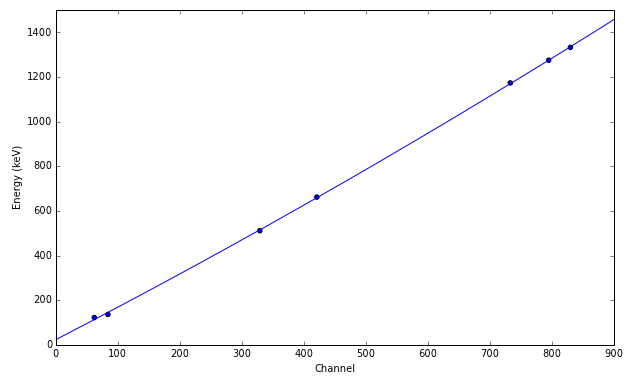
\includegraphics[width=\textwidth]{Calibrate.png}
\caption{Known photopeak values for $^{57}$Co, $^{137}$Cs, $^{2}$Na, and $^{60}$Co compared against the measured channel numbers determined from the MCA}
\label{Calibrate}
\end{figure}

\begin{table}[h]
\caption{Measured and known photopeak and backscatter peak energies from gamma-ray sources.}
\begin{ruledtabular}
\begin{tabular}{c c c c c}
&Source&$E_{measured}$ (keV)&$E_{known}$ (keV)&
\\
\hline
 &$^{60}$Co&1169 $\pm$ 3 &1173.2&\\
&$^{60}$Co&1335 $\pm$ 3&1332.5&\\
 &$^{57}$Co&113$\pm$ 9&122.1&\\
&$^{57}$Co&145$\pm$ 9&136.0&\\
&$^{137}$Cs&659$\pm$ 2&661.7&\\
&$^{22}$Na&515$\pm$ 4&511.0&\\
&$^{22}$Na&1275.1$\pm$ .1&1275.0&\\
\end{tabular}
\end{ruledtabular}
\label{Energies}
\end{table}

\newpage
More detailed information was gathered on $^{137}$Cs; the full width at half maximum for its photopeak was determined to be 46$\pm6$ keV, while it's Compton edge and peak associated with Compton backscattering were determined to have energies of 469$\pm3$ keV and 220$\pm8$ keV respectively. The theoretical Compton edge value of 474.772$\pm0.001$ keV is in agreement with the measured value presented here. The angle of the incident gamma rays which produced the Compton backscattering peak were calculated to be 122.97$\pm0.02$ degrees.

\subsection{Resolution}
The resolution of the photopeak on $^{137}$Cs was calculated to be 0.070$\pm0.002$ using the method described in subsection C of the Experimental Design. Additionally, using that same method, the resolution of $^{60}$Co was found to be 0.065$\pm0.001$. With these two values we can show the correctness of the theoretical value of $-1/2$ for $x$ in the proportionality from Eq. \eqref{proportionality}. We do this by comparing the ratio of the resolutions for $^{60}$Co and $^{137}$Cs to the theoretical ratio based upon the measure values for $E_{Co}$, $E_{Cs}$ and theoretical value for $x$. By this method we find the measured resolution ratio to be 0.93$\pm0.03$ and the calculated ratio to be 0.70$\pm0.02$. Thus the two values are not in agreement.

\subsection{Identification of an Unknown Isotope}
After selecting an unknown radioactive Isotope, the photopeak which the radiation produced was measure with the PMT and MCA and then calibrated using the calibration function described in Eq. \eqref{calib}. The measured value of the photopeak was determined to be 829$\pm3$ keV. Then, using the 8th Edition of the Table of Isotopes which was last updated in 1999, and filtering through it by reviewing isotopes with half-lives greater than 1 hour, a single likely candidate, which most closely matched our photopeak measurement, was identified as being $^{54}$Mn. This isotope has an 834.848 keV photopeak and 312.3 day half-life \cite{isotopes}. In comparing the two values we find that the photopeak energy for the selected element in the table of isotopes is in agreement with our own measured value.

\section{Conclusion}
This report utilizes scintillators and a PMT MCAto analyze the details of radioactive isotopes through the gamma-rays emitted with each decay. In doing so we perform the kinds of analysis that Marie Curie, and other like her who studied these materials in the late 1800's and 1900's, could only have dreamed of. Here we detail our analysis of the radioactive isotopes $^{57}$Co, $^{137}$Cs, $^{22}$Na, and $^{60}$Co in addition to another unknown Isotope which sought to identify. The photopeak energies for these elements reported in keV were found to be 113$\pm9$, 659$\pm2$, 1275.1$\pm0.1$, 1169$\pm3$, and 829$\pm3$ respectively. Their corresponding accepted values, also reported in keV, are 122.1, 661.7, 1275.0, and 1173.2 with the exception of the unknown. A comparison of these values, again with the exception of the unknown, showed that all the measured values are in agreement with their analogous accepted values. A more extensive examination of $^{137}$Cs showed that the full width at half maximum of its photopeak was 46$\pm6$ keV, with a Compton edge of 469$\pm3$ keV, and secondary peak energy of 220$\pm8$ keV. The theoretical Compton edge value of 474.772$\pm0.001$ keV is shown to be in agreement with the measured value presented here. The secondary peak was identified as an artifact of Compton backscatter as the angle of the incident gamma-rays required to produce this peak was calculated to be 122.97$\pm0.02$ degrees. Additionally, the resolution of the photopeak on $^{137}$Cs was calculated to be 0.070$\pm0.002$ and the resolution of $^{60}$Co's photopeak was found to be 0.065$\pm0.001$. Finally, using the 8th Edition of the Table of Isotopes which was last updated in 1999, to compare the known and measured photopeak energies, $^{54}$Mn was found to match the energy spectrum of our unidentified isotope. The known photopeak for $^{54}$Mn is 834.848 keV while the measured photopeak of unknown, previously listed, was 829$\pm3$ keV. In comparing the two values we find that the photopeak energy for the identified element in the table of isotopes is in agreement with our own measured value for the unknown isotope.

\newpage

\begin{acknowledgments}

Thank you to my esteemed colleagues who agreed with me when I proposed more large explosions in the report as an answer to its technical flaws. Though my editor would not allow the changes I acknowledge our seemingly subliminal connection.

\end{acknowledgments}


\begin{thebibliography}{99}

\bibitem{scin}  Glasser, Otto (1933). Wilhelm Conrad R�ntgen and the Early History of the Roentgen Rays. London: John Bale, Sons and Danielsson, Ltd. p. 305.

\bibitem{curie} Mould, R. F. (1998). ``The discovery of radium in 1898 by Maria Sklodowska-Curie (1867--1934) and Pierre Curie (1859--1906) with commentary on their life and times". The British Journal of Radiology \textbf{71} (852): 1229--54.

\bibitem{isotopes} Richard B. Firestone, S.Y. Frank Chu, Coral M. Baglin ``8th edition of the Table of Isotopes: 1999 Update" John Wiley \& Sons Inc., (1999).

\bibitem{R}  R. Hofstadter, IEEE Trans. Nucl. Sci. NS-22 (1975) 13.

\end{thebibliography}

\end{document}
